\section{Umsetzung}
\label{umsetzung}
%Wenn die verwendete Linux-Distributon einen Paketmanager unterstützt 
Unterstützt die verwendete Linux-Distribution einen Paketmanager verläuft die Installation der Anwendung einfach und ohne Probleme.
%Die Installation der Anwendung verläuft einfach und ohne Probleme.
Die hier als Testserver eingesetzte Ubuntu-Distribution verknüpft automatisch die Munin-Webseiten mit dem Webserver und verlinkt bereits die ersten verwendbaren Munin-Plugins.
Aus diesem Grund sind sofort nach der Installation einige Graphen verfügbar, siehe Abbildung \ref{ootb}.

\begin{figure}[ht]
	\centering
	   \fbox{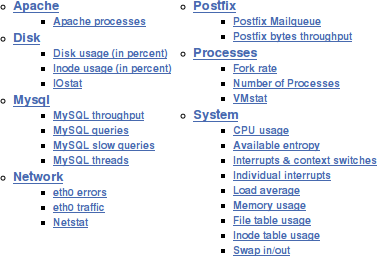
\includegraphics[width=0.8\textwidth]{bilder/ootb.png}}
		\caption{Bereits nach der Installation verfügbare Munin-Graphen}
		\label{ootb}
\end{figure}

Dabei untersucht Munin das verwendete System während der Installation nach verfügbaren Überwachungssobjekten.
Zum Beispiel wurde in der oberen Abbildung von Munin der Mailserver \textit{postfix} gefunden und automatisch in eine eigene Kategorie in das Webinterface eingepflegt.

Wie bereits in Kapitel \ref{plugins} beschrieben können weitere mitgelieferte Munin-Plugins in das entsprechende Service-Verzeichnis verlinkt und dabei ggf. mit Parametern ausgestatten werden, damit Munin zusätzlich diese Graphen erstellt und deren Werte aktualisiert und abspeichert.

Dabei gibt es noch eine zusätzliche Hilfe durch die Plugins, sofern sie sich an den Munin-Plugin-Standard halten.
Solche Skripte überprüfen selbständig bei ihrer Ausführung unter welcher Bedingung sie nicht genutzt werden können oder mit welchen Parametern sie funktionieren würden.

Diese hilfreiche Unterstützung erhält man durch die Ausführung des folgenden Befehls:

\begin{figure}[ht]
	\centering
	   \fbox{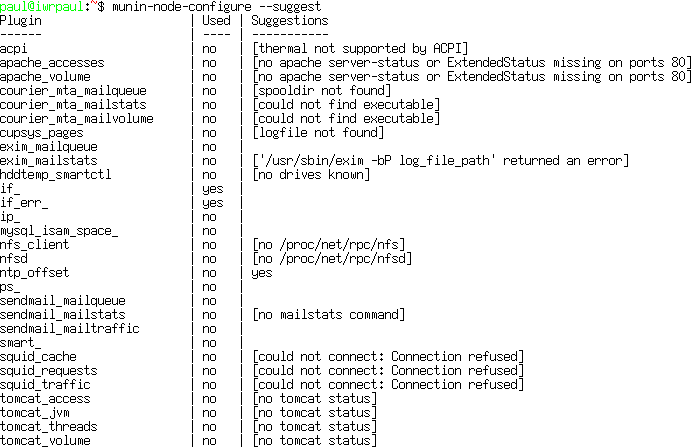
\includegraphics[width=0.9\textwidth]{bilder/suggest.png}}
		\caption{Automatische Überprüfung der Munin-Plugins}
		\label{suggest}
\end{figure}

Anhand dieser Informationen kann herausgefunden werden, weshalb ein Plugin nicht richtig funktioniert oder nicht automatisch bei der Installation hinzugefügt wurde.
\newpage
\subsection{Erstellen eines eigenen Munin-Plugins}

Die zum Zeitpunkt dieser Arbeit mitgelieferten 132 Munin-Plugins unterstützen eine Vielzahl an verschiedenen Überwachungsmöglichkeiten.
Es kann jedoch auch sein, dass ein gewünschtes Element oder Detail nicht von den mitgelieferten Plugins beachtet wird.
Dann bietet es sich an auf der MuninExchange\footnote{http://muninexchange.projects.linpro.no/} Internetseite nach bereits entwickelten, passenden Munin-Plugins zu stöbern.

Eine weitere Möglichkeit besteht darin das gewünschte Skript selbst zu entwickeln.
Da der Aufbau eines Munin-Plugins recht primitiv und klein ausfallen kann, benötigt man keine umfangreichen Programmierkenntnisse um erfolgreich ein funktionierendes Skript zu entwickeln.

Im Folgenden soll als Beispiel eine einfache Speicherplatzüberwachung eines Ordners mit Munin realisiert werden.

Dafür wird das bereits vorhandene Systemtool \textit{du} verwendet.
Der Speicherplatzbedarf eines Ordners lässt sich dann folgendermaßen ermitteln:

\begin{figure}[ht]
	\centering
	   \fbox{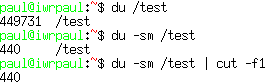
\includegraphics[width=0.55\textwidth]{bilder/du1.png}}
		\caption{Ermittlung des Speicherplatzbedarf des Ordners \textit{/test}}
		\label{du1}
\end{figure}

Mit dem ersten Befehl wird die Verzeichnisgröße des Ordners \textit{/test} gemessen.
Der dabei ermittelte Rückgabewert besitzt KByte als Einheit; da es sich aber um einen etwas größeren Ordner handelt und damit der spätere Munin-Graph nicht zu unübersichtlich wird, bietet es sich an, diese Einheit mit dem zweiten Befehl durch den zusätzlichen Parameter \textit{-sm} in MByte umzurechnen.
Da nur der Speicherplatzbedarf des Ordners interessiert, wird der zweite Teil der Ausgabe mit dem \textit{cut}-Befehl abgeschnitten.

Eine für Munin verwertbare Ausgabe, wie in Abbildung \ref{df-munin}, muss einen internen Variablennamen, in diesem Fall \textit{dir}, gefolgt von dem Suffix \textit{.value}, besitzen.
Daraus ergibt sich folgendes BASH-Skript:

\begin{lstlisting}[captionpos=b, caption=Speicherplatzbedarf eines Verzeichnisses, label=du, breaklines = true, language=bash]
#!/bin/bash
# Plugin to monitor the size of the specified directory
#
# directory to check
DIR="/test"

echo -n "dir.value "
if [ -d $DIR ]; then #check if the dir exists
    SIZE=`du -sm $DIR | cut -f1`
    echo $SIZE
    exit 0
else
    echo "Error: check your directory!"
    exit 1
fi
\end{lstlisting}

Nach der Verlinkung in das entsprechende Service-Verzeichnis gibt das Skriptes folgende Ausgabe zurück:

\begin{figure}[ht]
	\centering
	   \fbox{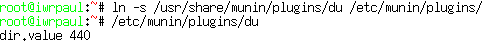
\includegraphics[width=0.85\textwidth]{bilder/du2.png}}
		\caption{Ausführung des Testplugins}
		\label{du2}
\end{figure}

Mit dieser Ausgabe kann \pictext{munin-update} die Messwerte ermitteln und speichern.

Für die Visualisierung dieser Messwerte benötigt Munin zusätzlich noch Informationen, wie der Graph auszusehen hat.
Um diese Informationen zu erhalten, ruft Munin die Plugins mit dem Parameter \textit{config} auf; daher muss auch dieses Plugin die entsprechende Werte bei diesem Parameteraufruf liefern.

Folgende Informationen werden für das Testplugin benötigt:

\begin{itemize}
\item \textit{graph\_title} als Titel für den Graphen
\item \textit{graph\_vlabel} als Beschriftung der y-Achse
\item \textit{graph\_category} für die Kategorie in welche der resultierende Graph eingeordnet werden soll
\item \textit{dir.label} als Bezeichnung der Messwerte
\item \textit{dir.min} als Minimalwert der Messwerte
\item \textit{dir.info} zusätzliche Beschreibung unterhalb des Graphen
\end{itemize}

Der dafür benötigte Quelltext wird vor der eigentlichen Messwertermittlung eingeschoben, da sich das Skript ansonsten zuvor mit \textit{exit} beendet.
Das fertige Skript sieht dann folgendermaßen aus:

\begin{lstlisting}[captionpos=b, caption=Fertiges Skript für den Speicherplatzbedarf eines Verzeichnisses, label=du, breaklines = true, language=bash]
#!/bin/bash
# Plugin to monitor the size of the specified directory
#
# directory to check
DIR="/test"

if [ "$1" = "config" ]; then
	echo "graph_title Directory size: $DIR"
	echo "graph_vlabel size MB"
	echo "graph_category disk"
	echo "graph_info Size of $DIR"
	echo "dir.label size"
	echo "dir.min 0"
	echo "dir.info Shows du -sm for specified directory"
	exit 0
fi

echo -n "dir.value "
if [ -d $DIR ]; then #check if the dir exists
    SIZE=`du -sm $DIR | cut -f1`
    echo $SIZE
    exit 0
else
    echo "Error: check your directory!"
    exit 1
fi
\end{lstlisting}

Nach dem Neustarten des \pictext{munin-node}-Daemons wird folgender Graph im Webinterface angezeigt:

\begin{figure}[ht]
	\centering
	   \fbox{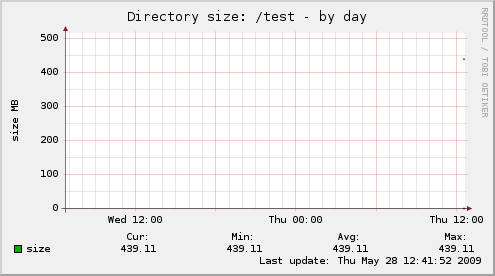
\includegraphics[width=0.85\textwidth]{bilder/du-graph.png}}
		\caption{Fertiger Muningraph des Testskriptes}
		\label{du-graph}
\end{figure}

Dies ist nur ein simples Beispiel für ein eigenes Munin-Plugin.
Dem Entwickler sind aber fast keine Grenzen gesetzt, solange er sich an die von Munin benötigten Werte hält.